\chapter{Estado del Arte}
\label{chapter:Estado del Arte}

Una de las aplicaciones más comunes dentro de la detección de anomalías es para la detección de intrusos (\textit{Intrusion Detection}) y la creación de sistemas de detección de intrusos (\textit{Intrusion Detection System, IDS}). Se trata de sistemas cuyo objetivo es la monitorización de los sistemas y redes informáticas, con el fin de alertar en caso de que puedan existir brechas de seguridad\cite{intrusionSystems}. 

Con la ingente cantidad de redes y sistemas que se pueden encontrar a día de hoy es necesario incluir uno de estos sistemas, con el fin de mantener la integridad y disponibilidad de los mismos. Dentro de los IDS, se pueden identificar dos grandes implementaciones de estos sistemas, en los sistemas de detección de intrusos en Host (\textit{Host-Based Intrusion Detection Systems, HIDS}) y los sistemas de detección de intrusos en red (\textit{Network Intrusion Detection Systems, NIDS}).

\begin{itemize}
    \item \textbf{HIDS:} Estos sistemas se caracterizan por implementarse en el Host utilizando información del propio sistema operativo para detectar actos maliciosos \cite{HIDS}. Esta información tiene distintos niveles de información, pero por lo general tienden a ser de bajo nivel sobre operaciones que se pueden estar realizando dentro del sistema. Esta información se consulta dentro de logs, por lo que el análisis de la información es más lento.
   \item \textbf{NIDS:} Para el segundo caso la monitorización se realiza a sistema de red, es decir, de comunicaciones entre distintos nodos y la monitorización de los paquetes que viajan entre ellos \cite{intrusionSystems}. Esta información puede ser consumida en tiempo real, por lo que la reacción ante algún evento es más rápida que en los HIDS que necesitan revisar las acciones.
\end{itemize}

%%% SECTION
\section{Métodos tradicionales de detección de anomalías}
En la sección actual se describen algunos de los métodos tradicionales utilizados en IDS, tanto para HIDS como para NIDS.

\begin{itemize}
    \item Network Security Monitor (NSM):  se trata de uno de los primeros sistemas que permitió auditar el tráfico que circulaba dentro de la red \cite{surveyIDS}. El sistema escucha pasivamente dentro de la red y detecta si existe una conducta sospechosa al desviarse de patrones de conducta. La mayor parte de la monitorización se basa en protocolos estándar como \textit{telnet, ftp, TCP/IP, etc.} por lo que le permitía utilizar una gran cantidad de datos heterogéneos.
    \item State transition analysis (USTAT): el sistema parte de que el host en un momento se encuentra en un estado seguro y que según las acciones que se realizan sobre el mismo el host cambia de estado, hasta que llega a un estado en el que compromete la seguridad \cite{surveyIDS}. Este sistema analiza los estados por los que ha pasado la máquina desde el estado seguro al comprometido. 
    \item GrIDS: se trata de un IDS que utiliza un sistema de construcción de grafos basados en la red, donde cada nodo representa a un host y las aristas las conexiones entre los mismos. La representación gráfica de la actividad de la red permite ayudar al espectador en identificar qué está sucediendo \cite{surveyIDS}.
    \item Haystack: en este caso el IDS se ayuda de métodos estadísticos para la detección de anomalías, definiendo estrategias para usuarios y grupos, además de definir variables del modelo como variables gaussianas independientes \cite{garcia2009anomaly}. Para la detección se incluyen una serie de intervalos en los valores que en el momento que salen del rango normal, se calcula la distribución de probabilidades y si el \textit{score} o puntuación es demasiado grande se genera una alerta.
\end{itemize}

Los métodos/sistemas listados se desarrollaron durante los años noventa, la tecnología ha evolucionado desde entonces y los sistemas se han vuelto más complejos y más propensos a los ciberataques. Por ello, se han desarrollado nuevas técnicas que se apoyan en el uso de técnicas de minería de datos (\textit{Data Mining}) y las técnicas que se describirán a continuación de \textit{Machine Learning}.

\section{Machine Learning y la detección anomalías}

El \textit{Machine Learning} es una rama de la inteligencia artificial cuya premisa es hacer que la máquina aprenda una tarea sin haber sido específicamente programada para ello. El término fue descrito por Arthur L. Samuel en 1959 en un artículo en el que explica estudios de \textit{Machine Learning} aplicado al juego de las damas \cite{samuel2000some}, utilizando en una primera instancia métodos de aprendizajes más generales, como las redes neuronales de las que hablaremos más adelante, y otro métodos que tendrán que ser parametrizados para sus distintos usos.

La inteligencia artificial se puede entender como la inteligencia ejercida por las máquinas, al contrario que la inteligencia natural inherente a los humanos, que son capaces de realizar tareas cognitivas que permiten potenciar la resolución de las mismas e imitar comportamientos como el aprendizaje \cite{russell2016artificial}. Dentro de la inteligencia artificial se pueden encontrar distintas definiciones según si se centran en el razonamiento o en el comportamiento:

\begin{itemize}
    \item Actuar humanamente: este enfoque se basa en que las máquinas actúen como humanos más centrado en la interacción de máquinas con personas, más que en la resolución de problemas. Esta interacción se puede ver reflejada en el test ideado por Alan Turing en 1950, en el que se somete a la máquina "inteligente" a un interrogatorio realizado por un humano, donde éste no sabe que está hablando con una máquina, por lo tanto si es incapaz de detectar que se trata de una máquina esta ha actuado como un humano y puede considerarse inteligente.
    \item Pensar humanamente: esta vertiente se centra en imitar el pensamiento humano, entender cómo funcionan las mentes de los mismos y replicarlo en máquinas. Siguiendo esta corriente, si se consigue imitar el pensamiento humano, una máquina que resuelva el problema utilizará razonamientos humanos, en lugar de solucionar problemas a toda costa, independientemente de como lo realizan los humanos.
    \item Pensar racionalmente: basado en la lógica formal desarrollada en en siglos XIX y XX que permite formular los problemas en un lenguaje formal, utilizando el razonamiento matemático para resolver éstos.
    \item Actuar racionalmente: se centra en realizar el comportamiento más efectivo en un momento dado. Antes las distintas situaciones no siempre existe una acción correcta, pero si se puede llegar realizar una acción que minimice los riesgos.
\end{itemize}

Los enfoques mostrados conllevan sus propios enfoques filosóficos, sin embargo, han influenciado en gran medida a cómo se afrontan los problemas y cómo se han desarrollado las técnicas de inteligencia artificial que están en uso actualmente.

Como se ha comentado con anterioridad, el \textit{Machine Learning} es una rama de la inteligencia artificial, dentro de la cual existe otra rama, \textit{Deep Learning}. Las relaciones entre los términos se puede observar en la imagen \ref{fig:ai-ml-dl} y como la inteligencia artificial engloba ambas ramas.

\begin{figure}[ht]
	\centering
	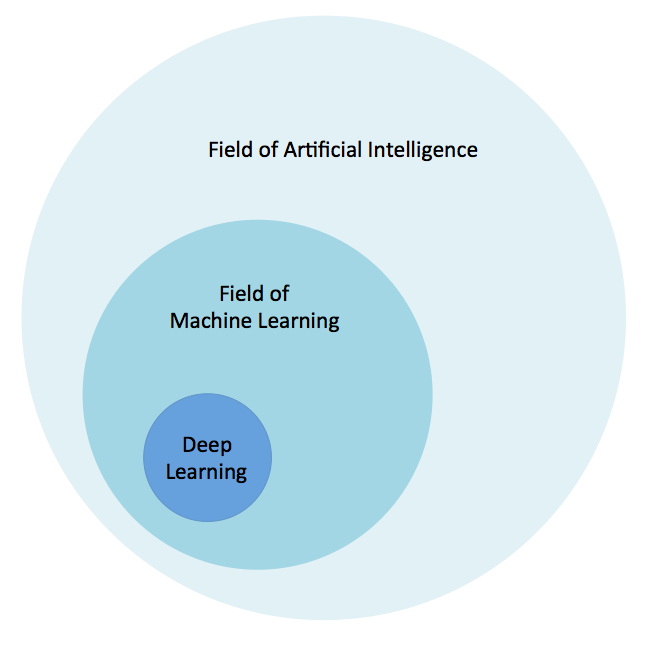
\includegraphics[width=8cm]{figs/ai-ml-dl-relationship.png}
	\caption{Relación entre Inteligencia Artificial, Machine Learning y Deep Learning}
	\label{fig:ai-ml-dl}
\end{figure}

El \textit{Deep Learning} se diferencia del \textit{Machine Learning} convencional, en que están formados por modelos con distintas ramas de procesamiento que son capaces de extraer las representaciones de los datos con varios niveles de abstracción \cite{lecun2015deep}. Mucha de la teoría relacionada se puede encontrar en los años 50 y 60, sin embargo, las aplicaciones y la capacidad de cómputo eran limitadas en la época, hasta ahora donde la capacidad de computación ha crecido a gran escala y en conjunto con las nuevas técnicas propuestas, una mayor cantidad de datos y la aplicación de transformaciones no lineales hacen que esta vertiente viva su época dorada.

Una de las implementaciones más representativas del \textit{Deep Learning} se trata de las redes neuronales, las cuales se encuentran basadas en el funcionamiento del cerebro humano, utilizando el concepto de neuronas que pueden realizar cálculos, la conexión entre las mismas, la función de realizar una tarea específica, etc. Añadir, que se encuentra basado y que el cerebro humano es un sistema mucho más complejo que las redes neuronales y tiene muchos más comportamientos \cite{haykin1994neural}.


Dentro del \textit{Machine Learning}, los algoritmos pueden dividirse según como se realice el entrenamiento del modelo, afectando también a la evaluación y las aplicaciones del mismo. Estas categorias son: \textit{Aprendizaje Supervisado (Supervised Learning), Aprendizaje No Supervidado (Unsupervised Learning) y Aprendizaje Semi-Supervisado (Semi-Supervised Learning)}

\subsection{Aprendizaje Supervisado}

El aprendizaje supervisado se caracteriza por utilizar un conjunto de variables de entrada y encontrar la función que más se aproxime a los valores de salida \cite{Liu2012}. Actualmente es una de las metodologías más utilizadas en \textit{Machine Learning} y es una de las más avanzadas en el campo, sin embargo, la necesidad de los valores de salida (variable dependiente o \textit{target}) requiere que el conjunto de datos se encuentre etiquetado, es decir, para las observaciones de las variables de entrada debe existir la variable de salida para poder general el modelo. En muchos casos este etiquetado se debe de realizar manualmente, por lo que es un proceso que requiere mucho tiempo.

Por otro lado, cabe mencionar que el uso de métodos de aprendizaje supervisado tienen una mayor efectividad que el semi y no supervisado, sin embargo, la necesidad de tener las etiquetas y el coste que ello supone para grandes cantidades de datos, como es en el caso de la detección de anomalías, provocan que se busquen otras soluciones con aprendizajes semi y no supervisado. Además, suele suceder que en la detección de anomalías, éstas sean la menor parte de todos los datos, en otras palabras, la mayor parte de los datos son normales y solo una pequeña porción se trata de anomalías como tal, provocando que el conjunto de datos esté poco compensado.

Uno de los modelos más sencillos de aprendizaje supervisado es la regresión lineal (simple), ésta permite ajustar a una serie de puntos conocidos , \textit{x}, y su respuesta \textit{y} \cite{james2013introduction}, generando una función que permite predecir los valores de \textit{y} con valores no conocidos de \textit{x}:

\begin{equation}
y = ax + b 
\end{equation}

En este caso se predicen los nuevos valores utilizando la función ajustada, existen distintos métodos para encontrar la recta que ajusta los puntos, siendo uno de los más utilizados el ajuste por mínimos cuadrados:

\begin{equation}
    a = \frac{\sum(x_i - \bar{x}) (y_i - \bar{y})} {\sum(x_i - \bar{x})^2}
\end{equation}

\begin{equation}
    b = y - a \bar{x}
\end{equation}

\begin{figure}[H]
	\centering
	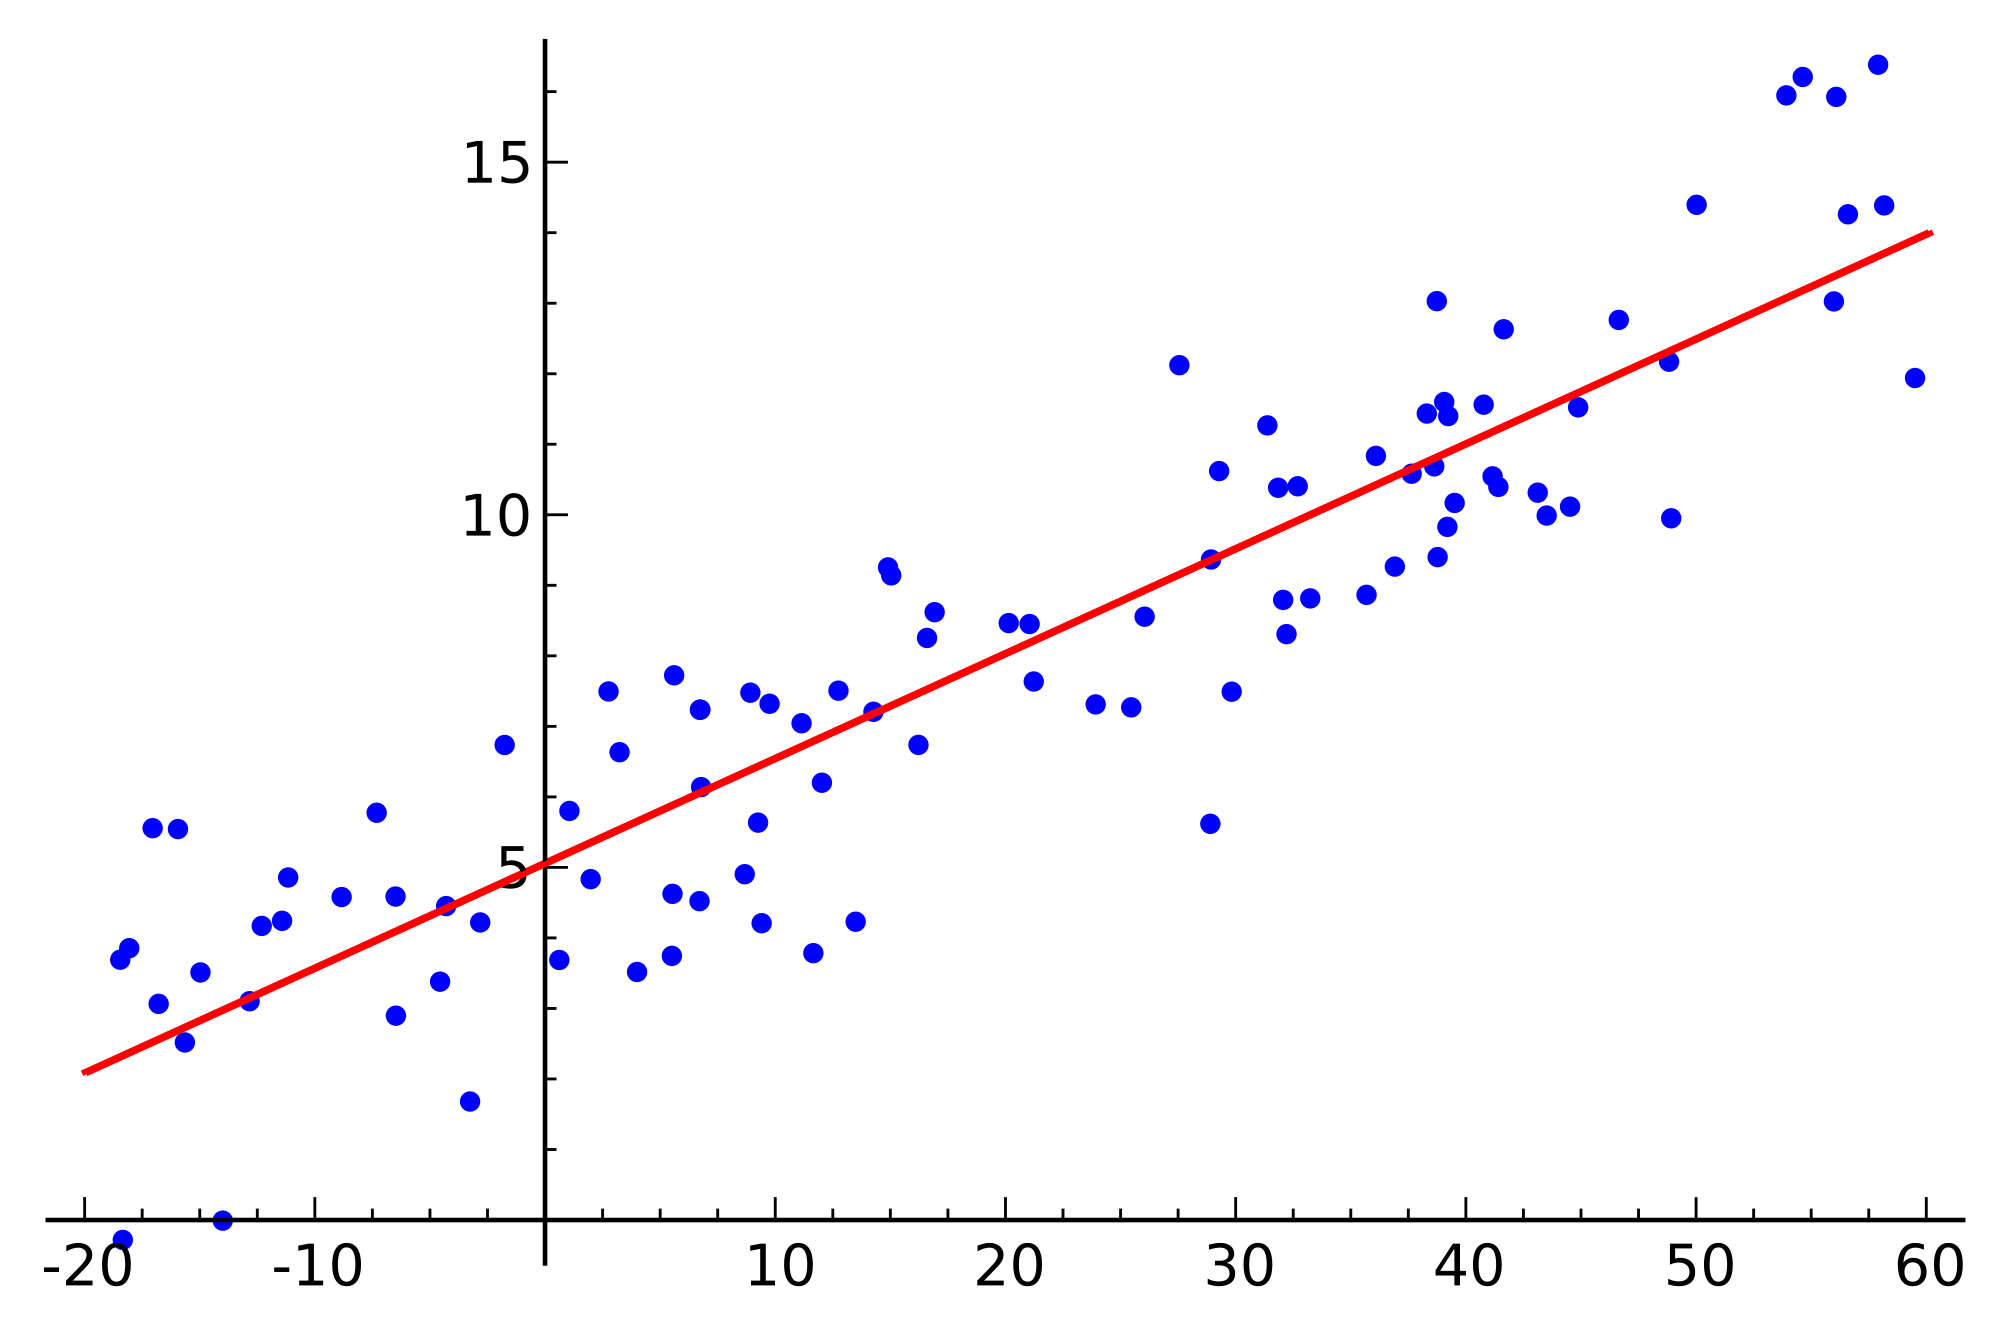
\includegraphics[width=8cm]{figs/Linear_regression.png}
	\caption{Regresión Lineal}
	\label{fig:reglin}
\end{figure}

Como se puede observar en la imagen \ref{fig:reglin}, se ha generado una recta capaz de ajustarse a los puntos y predecir el valor para nuevos puntos. Para generar la función de la recta se ha necesita utilizar la variable dependiente \textit{y} en el entrenamiento para poder generar la función que aproximará los nuevos puntos. 

Durante los siguientes apartados se van a mostrar los distintos modelos utilizados en aprendizaje supervisado para la detección de anomalías, como las redes neuronales artificiales (\textit{Artificial Neural Networks, ANN}, \textit{Gradient Boosting Machines} y \textit{Support Vector Machines}

\subsubsection{Feedforward Neural Network}

Tal y como se ha comentado anteriormente, las redes neuronales intentan imitar el concepto de la conexión de neuronas del cerebro humano, éstas están formadas por una capa de entrada de datos (\textit{Input}), una capa de salida (\textit{Input}) y un conjunto de capas intermedias, también llamadas capas ocultas (\textit{Hidden}) \cite{haykin1994neural}. En las capas intermedias se encuentran las neuronas conectadas entre sí y pueden estar formadas desde una sola capa, hasta \textit{n} capas, sin embargo, cuanto mayor sea el número de capas, mayor coste de computación asociado. En la siguiente imagen \ref{fig:ANN} podemos ver como sería una arquitectura de una red neuronal:

\begin{figure}[H]
	\centering
	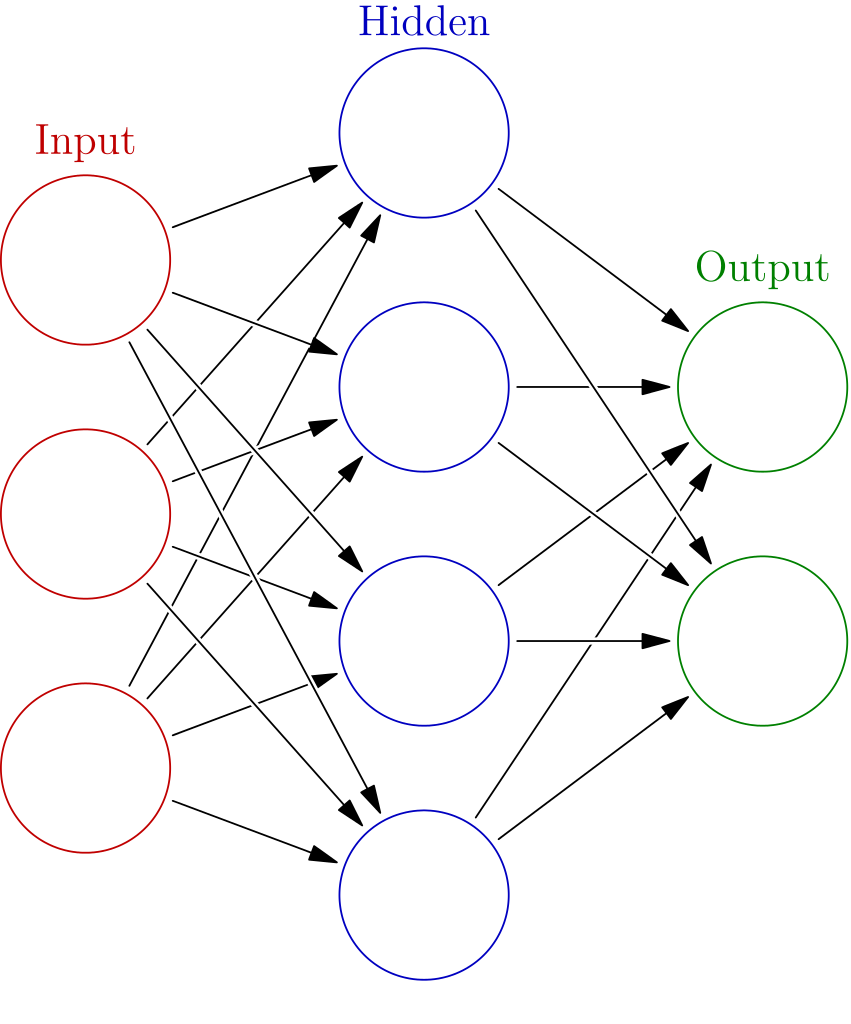
\includegraphics[width=8cm]{figs/Colored_neural_network.png}
	\caption{Red Neuronal Artificial}
	\label{fig:ANN}
\end{figure}

Dentro de las redes neuronales existe un caso base conocido como perceptron, un clasificador binario formado por la capa de entrada, una capa oculta de una sola neurona y una salida \cite{rosenblatt1958perceptron}. El perceptrón ayudará a incluir el concepto de los pesos (\textit{weights}) y el \textit{bias}. 

\begin{figure}[H]
	\centering
	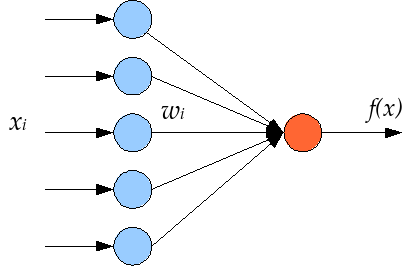
\includegraphics[width=8cm]{figs/Single_layer_perceptron.png}
	\caption{Arquitectura de un Perceptron}
	\label{fig:perceptron}
\end{figure}

Los valores de entrada \(X\) son multiplicados por una serie de pesos \(W\), en una primera instancia se inician aleatoriamente, y se realiza la suma de esta multiplicación, tras la cual se pasará a una función de activación. La función de activación define el valor de salida de la neurona y que se utilizará como valor de entrada para la siguiente neurona o como es en este caso como el valor de salida final. Un ejemplo de una función de activación es la función escalón, donde los valores menores de cero son iguales a cero y los mayores de cero son igual a uno. El \textit{bias} se trata de un pequeño valor que modifica el output sin interactura con las neuronas. De este modo la clasificación de 0 o 1 en un perceptron sería así:

\begin{equation}
    f(x) = g(\sum XW + b)
\end{equation}

Donde \(g(x)\) es la función de activación, X el vector de datos de entrada, W el vector de pesos y b el vector de bias.

\begin{figure}[H]
	\centering
	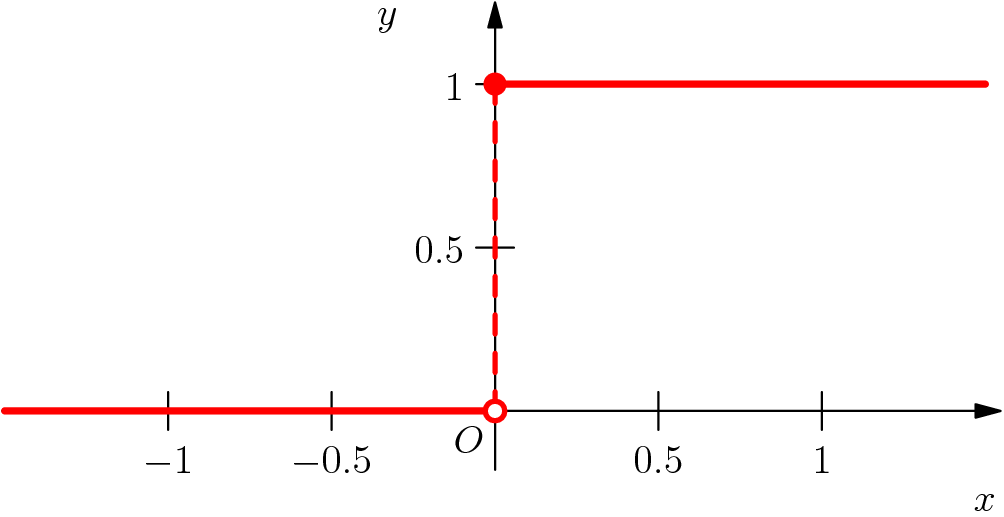
\includegraphics[width=8cm]{figs/stepfunction.png}
	\caption{Función de activación: Función Escalón}
	\label{fig:stepfunction}
\end{figure}

Aumentando la complejidad de la arquitectura, es decir, el número de neuronas, el numero de capas y distintas funciones de activación, se consiguen modelos más complejos pero mantienen el enfoque que se realiza en el perceptron.

Para optimizar la salida, se utilizan varias técnicas de optimización que permiten actualizar los pesos \(W\) y disminuir el error \(E = f(x) - y\), una de las más utilizadas es el \textit{backpropagation}, basado en el descenso del gradiente cuyo objetivo es obtener el gradiente de la función (vector de mayor pendiente) pero utilizar el valor opuesto del mismo multiplicado por un coeficiente de aprendizaje (\textit{learning rate}), una analogía muy utilizada es imaginar como encontrar el punto más bajo del valle, para ello lo mejor es fijarse en que lugar del punto en el que nos encontremos tiene más pendiente negativa y seguir ese camino. El backpropagation utiliza esté método, pero en lugar de calcular el gradiente sobre la función total (gran coste) se realiza el cálculo de los gradientes locales, empezando desde el punto final de la función.

\begin{figure}[H]
    \centering
    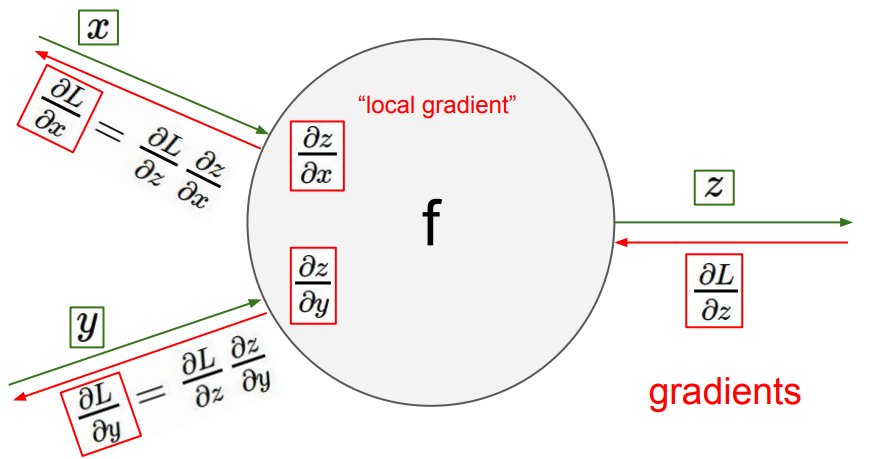
\includegraphics[width=8cm]{figs/backprop.png}
    \caption{Backpropagation}
    \label{fig:backprop}
\end{figure}

La fórmula de la actualización de los pesos en una ANN sería similar a la siguiente:
\begin{equation}
    W_{i+1} = W_i - \gamma d W
\end{equation}

Donde \(\gamma\) es el \textit{learning rate} y \(L(x)\) es la función de pérdida.

La última capa, la capa de \textit{outputs}, define el número de neuronas de salida, que puede ser igual al número de clases etiquetadas o una sola neurona en el caso de que existan solo dos clases, clasificación binaria. El valor de las salidas irá definido por la función de activación de la última capa de la capa oculta.

\subsubsection{Gradient Boosting Machines}

Las \textit{Gradient Boosting Machines} son uno de los métodos más utilizados actualmente, dada la gran precisión que aportan a la resolución de los problemas. Estos modelos se basan en realizar el ensamblado de modelos débiles, normalmente árboles de decisión, para generar un predictor "fuerte" de una manera iterativa. 

El término \textit{Boosting} se refiere al método utilizado para mejorar el aprendizaje de un modelo mediante el ensamblado de modelos débiles, esto quiere decir que son modelos con una capacidad de predicción mejor que la pura aleatoriedad \cite{freund1996experiments}. 

Concretamente el \textit{Gradient Boosting} trata de generar un primer árbol para realizar las predicciones, es decir, crea un función \(F(x)\) para aproximar \(y\), posteriormente se utiliza la función de coste definida (puede ser un error cuadrático medio para una regresión, por ejemplo) para ver como de bien ha realizado la predicción. Los residuales obtenidos se utilizan para crear un nuevo modelo que utilice estos residuales con el fin de volver a minimizar el error y finalmente se genera un nuevo modelo que utilice ambos. De esta forma en cada iteración su puede añadir \textit{n} cantidad de nuevos modelos que ayuden a mejorar las predicciones mediante la corrección de los errores de los modelos previos \cite{webgbm}.

Se crea el primer modelo
\begin{equation}
    F_1(x) = y
\end{equation}

Se crea un segundo modelo con los residuales
\begin{equation}
     h_1(x) = y - F_1(x)
     \label{eq:residuals}
\end{equation}

Se genera un nuevo modelo con los anteriores
\begin{equation}
     F_2(x) = F_1(x) + h_1(x)
\end{equation}

Dentro del ajuste a los residuales es donde entra la parte del gradiente, tal y como hemos explicado anteriormente se utiliza el método del descenso del gradiente (\textit{Gradient Descent}) para la optimización de la función de pérdida. Para cada paso que se realiza, en vez de calcular los residuales como en la fórmula \ref{eq:residuals} se ajustan calculando el gradiente de la función de pérdida y ajustando un nuevo modelo, \(h\), con los nuevos residuales y en la generación del nuevo modelo incluirle \textit{gamma} (\(\gamma\)), similar al concepto explicado de \textit{learning rate}:

\begin{equation}
    r = - [ \frac{\partial L(F(x_i),y)}{\partial F(x_i)} ]
\end{equation}

\begin{equation}
        F_2(x) = F_1(x) + \gamma h_1(x)
\end{equation}

En la práctica el uso de estos modelos se ha comprobado que es realmente eficaz para la resolución de problemas. Dentro de estos algoritmos se pueden destacar dos en concreto, cuyas implementaciones se han utilizado en varias soluciones dentro de las competiciones realizadas por Kaggle.

\textbf{XGBoost}

Diminutivo de \textit{eXtreme Gradient Boosting} se trata de una nueva implementación de GBM realizada por Chen, Tianqi, et al \cite{chen2016xgboost}, que demuestra una mayor escalabilidad y velocidad que los métodos tradicionales, utilizando una menor cantidad de recursos de los sistemas.  

\textbf{LightGBM}

Desarrollado por Microsoft \cite{ke2017lightgbm} se propone mejorar los problemas encontrados en algoritmos como \textit{XGBoost} cuando existe una alta cantidad de variables, esto es ocasionado por la necesidad de evaluar el punto óptimo para la división de los árboles de decisión. Propone su propia forma de efectuar la ganancia de información (por división) y demuestra una mejora en el tiempo de cómputo sobre los modelos convencionales.

Algunas de las competiciones donde se han utilizado los algoritmos (también ensamblándolos) son las siguientes:

\begin{itemize}
    \setlength\itemsep{0.5cm}
    \item Home Credit Default Risk: Can you predict how capable each applicant is of repaying a loan? \cite{kagglehome}.
    \item Corporación Favorita Grocery Sales Forecasting: Can you accurately predict sales for a large grocery chain? \cite{kagglefav}.
    \item Google Analytics Customer Revenue Prediction: Predict how much GStore customers will spend \cite{kagglegoogle}.
\end{itemize}

\subsubsection{Support Vector Machines}

Se trata de otro algoritmo enfocado a la clasificación mediante la separación de los puntos por un hiperplano \cite{james2013introduction}. Por ejemplo, para un set de datos etiquetados con dos categorías (clasificación binaria) se busca encontrar la línea (hiperplano) que mejor separe ambos puntos, como puede observarse en la imagen \ref{fig:svm} existen distintos hiperplanos (\(H_1 , H_2 , H_3\)) que separan las distintas clases, como puedo observarse tanto \(H_1\) como  \(H_2\) son capaces de separar las dos clases por completo, mientras que \(H_3\) fallaría en la tarea de clasificación .


\begin{figure}[H]
    \centering
    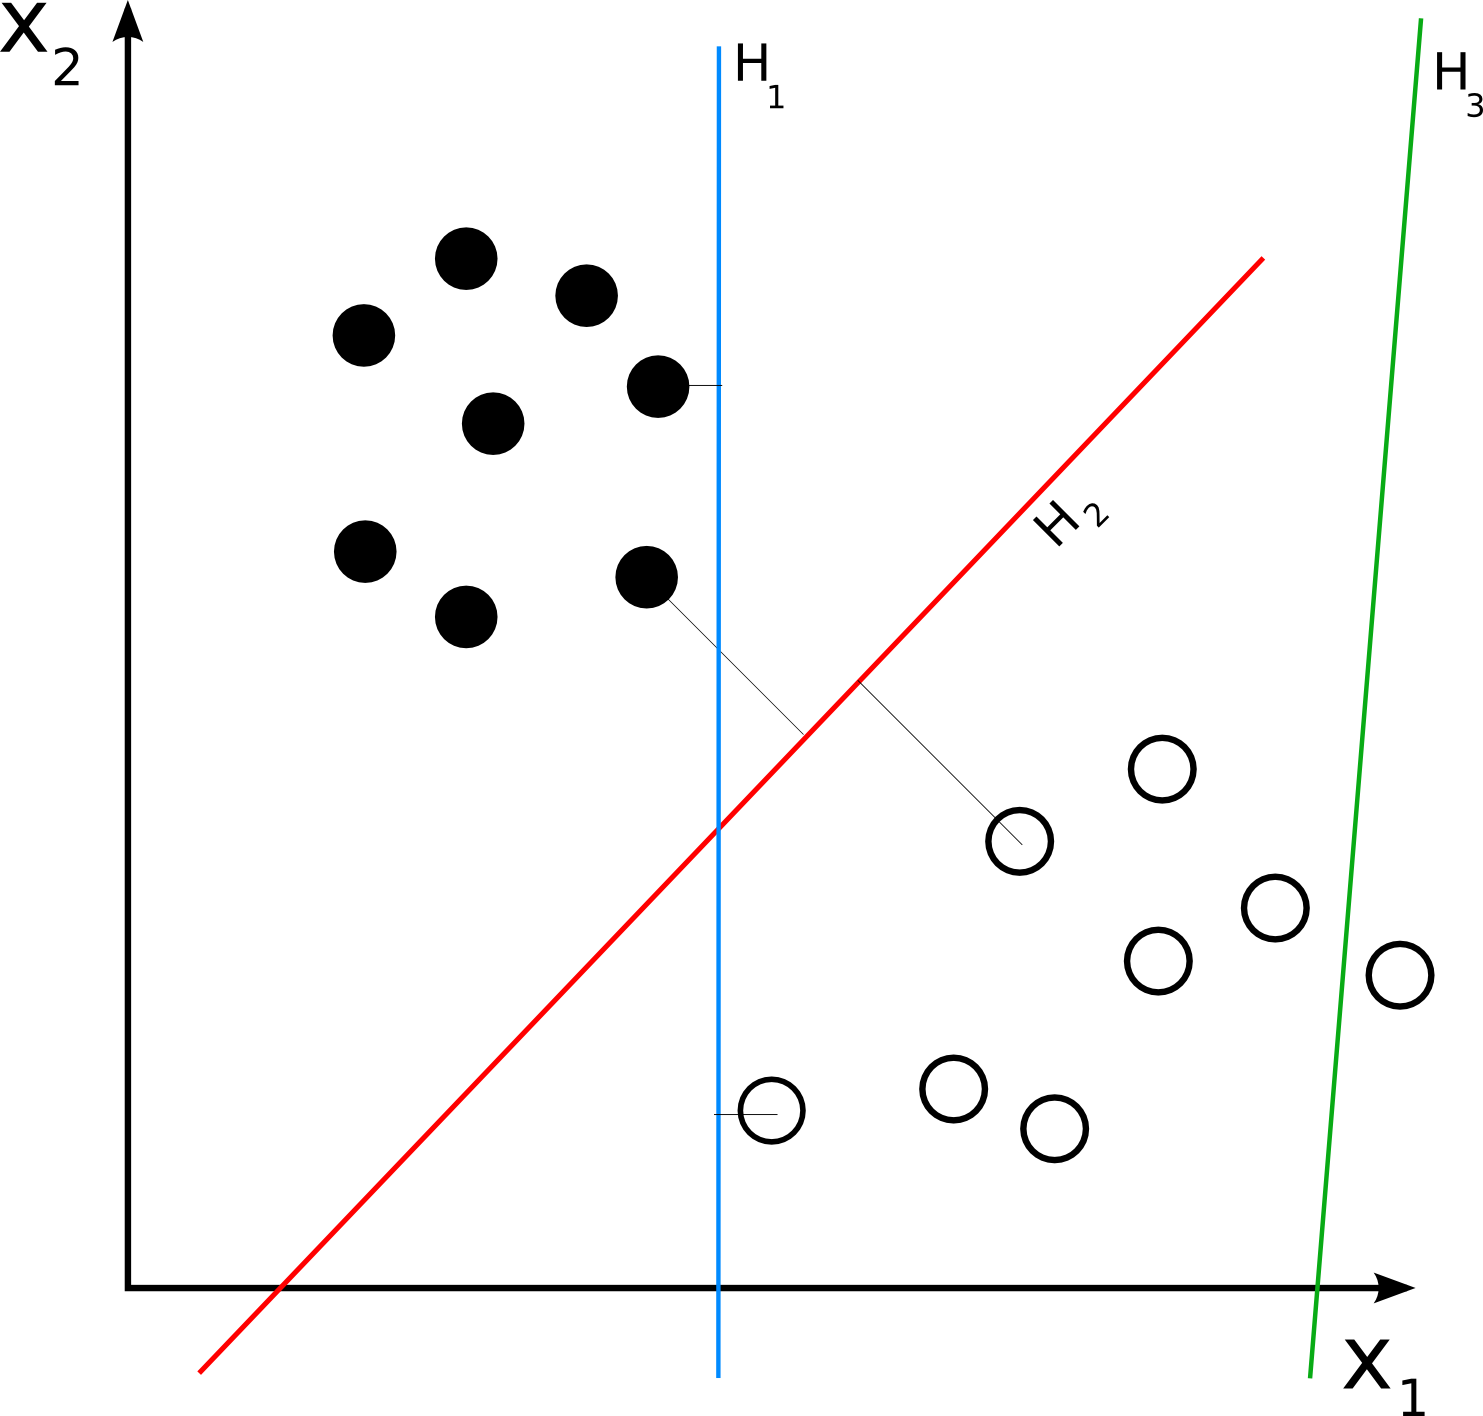
\includegraphics[width=8cm]{figs/Svm_separating_hyperplanes.png}
    \caption{Hiperplanos SVM}
    \label{fig:svm}
\end{figure}

Se puede definir el hiperplano como la "línea" que puede dividir los datos entre las dos clases, es decir, se pretende separar el espacio en dos mitades. Esta "línea" para un problema de \(p\) dimensiones sería de \(p-1\) dimensiones, en otras palabras, para un un problema de dos dimensiones sería una línea, para uno de tres sería un plano y así sucesivamente hasta \(n\) dimensiones. Esta separación indica que según donde se encuentren los puntos con respecto al hiperplano se clasificarán como una clase u otra.

\begin{equation}
    \beta_0 + X_1\beta_1 + X_2\beta_2 +  ... +  X_n\beta_n = 0 
\end{equation}

Como se ha mencionado en la imagen \ref{fig:svm}, existen varios hiperplanos, sin embargo, se debe de buscar el hiperplano óptimo de los posibles, siendo este el que se encuentra más alejado de los puntos de entrenamiento, es decir, es el hiperplano con mayor margen entre los puntos y el hiperplano. Sin embargo, si solo nos basamos en encontrar el mejor hiperplano según los márgenes se puede dar el caso de que un nuevo punto afecte en gran medida al hiperplano, por maximizar los márgenes, por ello se utiliza un parámetro \textit{C} que permite "ablandar" el clasificador y permitir que ciertos puntos puedan encontrarse entre el hiperplano y el margen, la mala clasificación de unos poco puntos permitidos evita sobreentrenar el modelo y permitir generalizar mejor.

\begin{figure}[H]
    \centering
    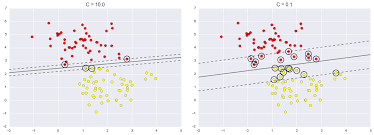
\includegraphics[width=11cm]{figs/svm_c.png}
    \caption{Hiperplanos para distintos valores de \textit{C}}
    \label{fig:svm_c}
\end{figure}

Por ahora, se ha hablado de separar los datos linealmente y en dos clases, sin embargo, ese no es siempre el caso, podemos tener más de dos clases o por ejemplo tenemos datos que no sean separables por una "línea", pensemos en dos conjuntos de puntos que forman una serie de circunferencias concéntricas (\ref{fig:svm_radial}), para este caso una línea nunca logrará separar bien los puntos. Para está última, la \textit{SVM} puede utilizar los \textit{kernels}, se trata de funciones que permiten cambiar la dimensionalidad del espacio para ayudar a la separación de las clases.

\textit{Kernel} lineal
\begin{equation}
    K(x_i, x_{i'}) = \sum_{j=1}^{p} x_ij x_{i'j}
\end{equation}

\textit{Kernel} polinomial
\begin{equation}
    K(x_i, x_{i'}) = (1 + \sum_{j=1}^{p} x_ij x_{i'j})^d
\end{equation}

\textit{Kernel} radial
\begin{equation}
    K(x_i, x_{i'}) = exp(-\gamma \sum_{j=1}^{p} (x_ij x_{i'j})^2)
\end{equation}

\begin{figure}[H]
    \centering
    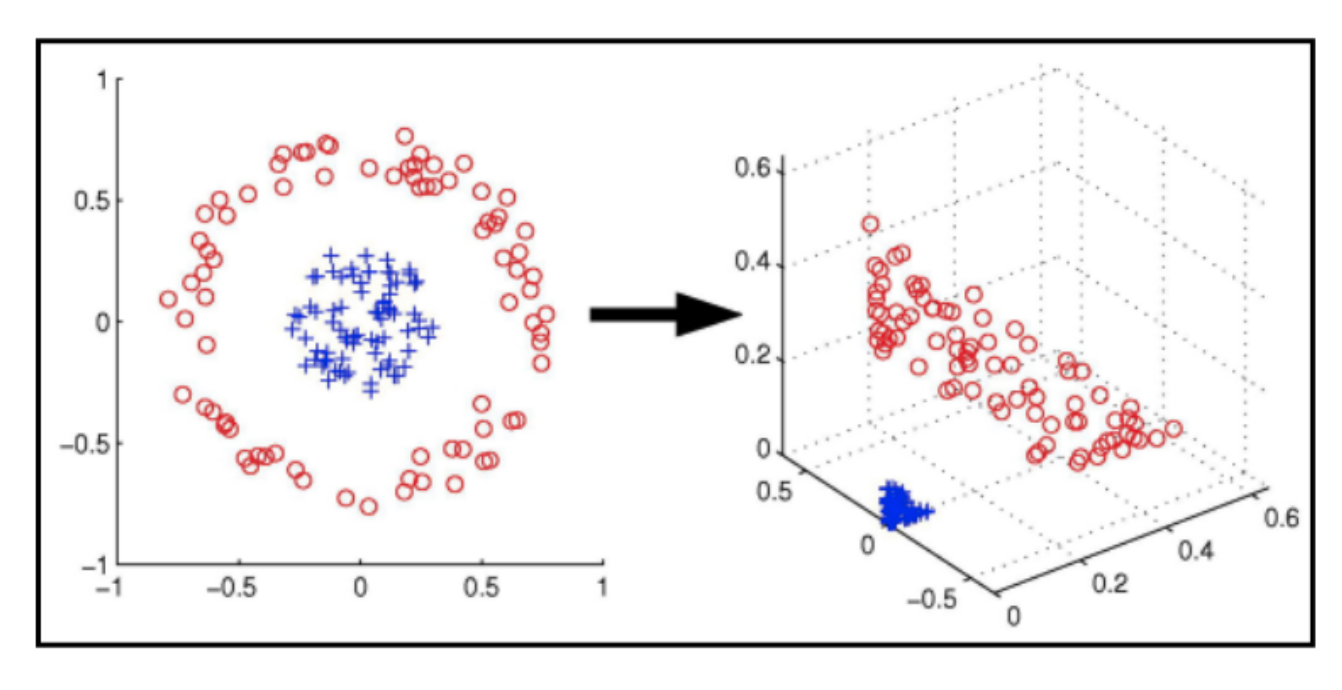
\includegraphics[width=8cm]{figs/svm_radial.png}
    \caption{Efecto de aplicación de \textit{Kernel} radial en SVM}
    \label{fig:svm_radial}
\end{figure}

Para el caso de tener más de dos clases se pueden aplicar dos enfoques distintos:

\begin{itemize}
    \item Clasificación uno contra uno: para este caso se crean una SVM por cada par de clases y realiza la clasificación para ellos, luego el resultado es elegido observando cuantas veces el punto cae en una categoría para las distintas SVM clasificándolo a la clase más frecuente.
    \item Clasificación uno contra todos: en este caso se realiza una SVM por clase, de modo que se compare la clase escogida con el resto y valorando en cual de los modelos generados es más apta la clasificación del punto.
\end{itemize}

\subsection{Aprendizaje No Supervisado}

Este nuevo tipo de aprendizaje se distingue porque no necesita ese conjunto de etiquetas que se utiliza por observación, es decir, en este caso no se tiene el valor de la clase o el valor numérico correspondiente a cierto conjunto de datos. Para este caso no se enfoca a la predicción de los valores, debido a que no tenemos esa variable \textit{target} para la que queremos desarrollar la función que la aproxime lo máximo posible, en este caso, el objetivo principal es intentar descubrir nuevos patrones o información oculta dentro de los datos \cite{james2013introduction}.

Muchas veces el uso del aprendizaje no supervisado no se encuentra con el simple objetivo de predecir, si no que puede ser parte de un proceso de análisis de los datos, de modo que permitan encontrar más información útil de los mismos, como por ejemplo, se puede realizar una segmentación de usuarios, de modo que posteriormente se pueda estudiar que causa esta segmentación de los mismos y mejorar los servicios que se les puedan ofrecer.

El uso del aprendizaje no supervisado esta creciendo cada vez más, dado que en la mayor parte de los casos los datos no vienen etiquetados, tal y como se ha comentado anteriormente el etiquetado de los mismos es un proceso costoso y además mientras que en el supervisado se puede "supervisar" si el resultado es correcto en la fase de entrenamiento, mientras que para el no supervisado, no se tiene esta capacidad de conocer cual es el valor real, dado que es imposible saber cual es la respuesta correcta.
\subsubsection{Análisis de Componentes Principales}
Se trata de uno de los algoritmos más conocidos cuya finalidad es explicar en una serie de "componentes", siendo la cantidad de éstos menor a la cantidad de variables de los datos iniciales, que permiten explicar la mayor parte de la varianza de los datos originales. Estos "componentes" se trata de un conjunto de nuevas variables que son capaces de explicar una gran parte de la varianza de un conjunto mayor, en otras palabras, permite obtener gran parte de la varianza explicada en un dimensionalidad menor.

En las siguientes imágenes se ha utilizado un set de datos sintéticos de dos dimensiones, en el que se muestra como en la imagen de la izquierda \ref{Fig:PCA1} se encuentran nubes de datos que cambian en función de los ejes \textit{x} e \textit{y} y como la aplicación del análisis de componentes principales \ref{Fig:PCA2}, \textit{PCA} de ahora en adelante, genera nuevas variables (dos componentes principales) que tienden a explicar la varianza de las variables originales. En este caso se puede apreciar como la aplicación del algoritmo "mueve" las observaciones, haciendo que así sean más identificables en a lo largo de los ejes.

\begin{figure}[H]
   \begin{minipage}{0.48\textwidth}
     \centering
     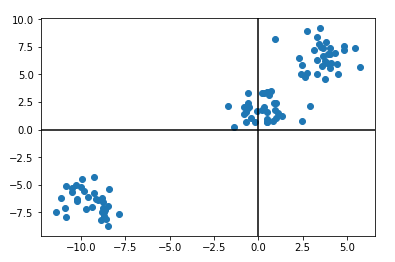
\includegraphics[width=1\linewidth]{figs/PCA_previo.PNG}
     \caption{Datos de dos variables sin PCA}
     \label{Fig:PCA1}
   \end{minipage}\hfill
   \begin{minipage}{0.48\textwidth}
     \centering
     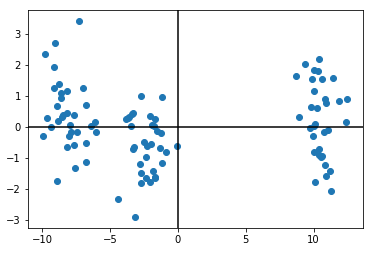
\includegraphics[width=0.95\linewidth]{figs/PCA_aplicado.PNG}
     \caption{PCA aplicado a dos variables}
     \label{Fig:PCA2}
   \end{minipage}
\end{figure}

Este ejemplo se trata de un caso sencillo, por lo general esta técnica también se puede utilizar para visualizar los datos de una gran dimensionalidad en dos o tres variables, utilizando ese número de componentes principales, que se tratan de una combinación lineal de las variables anteriores \cite{james2013introduction}.

Para realizar el cálculo del PCA, se puede realizar mediante el uso de álgebra lineal, más en concreto con una descomposición de autovalores y autovectores que siguen los siguientes pasos para una matriz \(X\) con \textit{p} variables y \textit{n} observaciones \cite{PCAscratch}:

Se calcula la media de cada una de las columnas
\begin{equation}
    \overline{X} = \overline{X_1}, \overline{X_2}, ... \overline{X_p} 
\end{equation}

Se normaliza el valor de las columnas restando la media de cada columna a todos los valores de la matriz

\begin{equation}
    X_(norm) = X - \overline{X}
\end{equation}

Se genera la matriz de covarianza con la matriz normalizada, siendo E la media, por cada par de variables \cite{covWikipedia}

\begin{equation}
    Cov[X_i, X_j] = E[(X_i - E[X_i])(X_j - E[X_j])]
\end{equation}

De la matriz de covarianza se calculan los autovalores y autovectores
\begin{equation}
    \lambda, \nu <- X_(cov)
\end{equation}

Una vez obtenidos los autovectores y autovalores, se seleccionarán un cantidad \textit{m} que será la cantidad de componentes principales elegidos

\begin{equation}
    B =  [\lambda_1 ... \lambda_m, \nu_1 ...\nu_m ]
\end{equation}

Y con estos calculamos la proyección \textit{P} de la matriz original \textit{X} con \textit{m} componentes principales

\begin{equation}
    P = B^T . A
\end{equation}

\subsubsection{Agrupación}
\subsubsection{Autoencoders}
\subsubsection{Generative Adversarial Networks}

\subsection{Aprendizaje Semi-Supervisado}
\subsubsection{Autoencoders}
\subsubsection{Convolutional Neural Networks}
\subsubsection{Generative Adversarial Networks}